\documentclass[sigconf, authordraft]{acmart}

\usepackage{booktabs} % For formal tables


% Copyright
%\setcopyright{none}
%\setcopyright{acmcopyright}
%\setcopyright{acmlicensed}
\setcopyright{rightsretained}
%\setcopyright{usgov}
%\setcopyright{usgovmixed}
%\setcopyright{cagov}
%\setcopyright{cagovmixed}


% DOI
\acmDOI{10.475/123_4}

% ISBN
\acmISBN{123-4567-24-567/08/06}

%Conference
\acmConference[WOODSTOCK'97]{ACM Woodstock conference}{July 1997}{El
  Paso, Texas USA}
\acmYear{1997}
\copyrightyear{2016}

\acmPrice{15.00}

\acmSubmissionID{123-A12-B3}

\begin{document}
\title{SIG Proceedings Paper in LaTeX Format}
\titlenote{Produces the permission block, and
  copyright information}
\subtitle{Extended Abstract}
\subtitlenote{The full version of the author's guide is available as
  \texttt{acmart.pdf} document}


\author{Ben Trovato}
\authornote{Dr.~Trovato insisted his name be first.}
\orcid{1234-5678-9012}
\affiliation{%
  \institution{Institute for Clarity in Documentation}
  \streetaddress{P.O. Box 1212}
  \city{Dublin}
  \state{Ohio}
  \postcode{43017-6221}
}
\email{trovato@corporation.com}

\author{G.K.M. Tobin}
\authornote{The secretary disavows any knowledge of this author's actions.}
\affiliation{%
  \institution{Institute for Clarity in Documentation}
  \streetaddress{P.O. Box 1212}
  \city{Dublin}
  \state{Ohio}
  \postcode{43017-6221}
}
\email{webmaster@marysville-ohio.com}

\author{Lars Th{\o}rv{\"a}ld}
\authornote{This author is the
  one who did all the really hard work.}
\affiliation{%
  \institution{The Th{\o}rv{\"a}ld Group}
  \streetaddress{1 Th{\o}rv{\"a}ld Circle}
  \city{Hekla}
  \country{Iceland}}
\email{larst@affiliation.org}

\author{Lawrence P. Leipuner}
\affiliation{
  \institution{Brookhaven Laboratories}
  \streetaddress{P.O. Box 5000}}
\email{lleipuner@researchlabs.org}

\author{Sean Fogarty}
\affiliation{%
  \institution{NASA Ames Research Center}
  \city{Moffett Field}
  \state{California}
  \postcode{94035}}
\email{fogartys@amesres.org}

\author{Charles Palmer}
\affiliation{%
  \institution{Palmer Research Laboratories}
  \streetaddress{8600 Datapoint Drive}
  \city{San Antonio}
  \state{Texas}
  \postcode{78229}}
\email{cpalmer@prl.com}

\author{John Smith}
\affiliation{\institution{The Th{\o}rv{\"a}ld Group}}
\email{jsmith@affiliation.org}

\author{Julius P.~Kumquat}
\affiliation{\institution{The Kumquat Consortium}}
\email{jpkumquat@consortium.net}

% The default list of authors is too long for headers.
\renewcommand{\shortauthors}{B. Trovato et al.}


\begin{abstract}
This paper provides a sample of a \LaTeX\ document which conforms,
somewhat loosely, to the formatting guidelines for
ACM SIG Proceedings.\footnote{This is an abstract footnote}
\end{abstract}

%
% The code below should be generated by the tool at
% http://dl.acm.org/ccs.cfm
% Please copy and paste the code instead of the example below.
%
\begin{CCSXML}
<ccs2012>
 <concept>
  <concept_id>10010520.10010553.10010562</concept_id>
  <concept_desc>Computer systems organization~Embedded systems</concept_desc>
  <concept_significance>500</concept_significance>
 </concept>
 <concept>
  <concept_id>10010520.10010575.10010755</concept_id>
  <concept_desc>Computer systems organization~Redundancy</concept_desc>
  <concept_significance>300</concept_significance>
 </concept>
 <concept>
  <concept_id>10010520.10010553.10010554</concept_id>
  <concept_desc>Computer systems organization~Robotics</concept_desc>
  <concept_significance>100</concept_significance>
 </concept>
 <concept>
  <concept_id>10003033.10003083.10003095</concept_id>
  <concept_desc>Networks~Network reliability</concept_desc>
  <concept_significance>100</concept_significance>
 </concept>
</ccs2012>
\end{CCSXML}

\ccsdesc[500]{Computer systems organization~Embedded systems}
\ccsdesc[300]{Computer systems organization~Redundancy}
\ccsdesc{Computer systems organization~Robotics}
\ccsdesc[100]{Networks~Network reliability}


\keywords{ACM proceedings, \LaTeX, text tagging}


\maketitle

\section{Introduction}

In the past decade, significant efforts have been made to implement the vision of the Semantic Web. Knowledge graphs (also called knowledge bases) such as DBpedia  \cite{lehmann2015dbpedia}, Freebase \cite{bollacker2007platform}, Google Knowledge Vault \cite{dong2014knowledge} or Yago \cite{suchanek2007yago} were created to provide access to structured data derived from various information sources. With the increasing usage of tools to extract structured data out of unstructured data, the Semantic Web is growing in the number of knowledge graphs being published and the size of already existing knowledge graphs. The value of these knowledge bases is intrinsically linked to the accuracy of the knowledge they represent. The demand for accurate facts in knowledge graphs grows continuously with the increased uptake of Linked Data.

One approach towards ensuring that knowledge bases contain reliable facts is the curation of facts in a knowledge base. While this task has been performed manually in the past~\cite{suchanek2007yago,gerber2015defacto}, the growth of knowledge bases in both size and number becomes increasingly prohibitive, as manual validation is both time-consuming and expensive given that it requires domain experts who can verify the facts. Hence, automatic algorithms that can check the validity of facts in a knowledge base have been devised over the last few years. Fact validation systems such as \DeFacto\ \cite{gerber2015defacto} rely on a web search engine to retrieve source documents for finding textual evidences. However, querying the Web frequently for information is a costly affair and might be subjective to the search engine. Moreover, reproducing consistent results is difficult due to continuous addition of new sources to the Web and the sustained adaptation of search engine results to user behaviour. 

In this paper, we present \FactCheck, an automated approach to validate RDF triples. \FactCheck is based on the same principles as \DeFacto\. Our algorithm takes an RDF triple as input and calculates a truth score by retrieving documents systematically from a given reference corpus and extracting sentences that express the input triple in natural language. However, \FactCheck{} relies on dependency parse trees and novel features for scoring how reliable RDF triples are. We evaluate the impact of our new approach to scoring triples by using two text corpora based on the English Wikipedia and ClueWeb12.\footnote{\url{https://lemurproject.org/clueweb09/}} We evaluate and report the results of \DeFacto\ and \FactCheck\ using the existing benchmark dataset FactBench \cite{gerber2015defacto} and a newly created dataset, which addresses some of the known weaknesses of FactBench. Our experiments show that %while both the algorithms achieved a better accuracy on ClueWeb, 
\FactCheck{} outperforms \DeFacto\ on all datasets with both reference corpora by up to 13.3\% F-measure and 19.3\% AUC

\section{Enhancements}
\label{sec:enhancements}
In this section, we present the extensions and enhancements we made to the existing \DeFacto\ as part of \FactCheck.% Wherever possible we make reference and differentiate with the \DeFacto.

\subsection{Local search engine}
One of the primary objectives of \FactCheck\ is to replace the Web search engine with a local search engine. Fact validation systems uses textual evidences extracted from relevant source documents for confirming facts. However, querying the Web for source documents is not an easy task. Developers rely on APIs provided by commercial search engines such as Google, Bing etc., which are typically not available for free. These APIs have limitations on their usage, for example the number of queries processed per user session. Moreover, there is less or no control on optimising search operations for performance and relevancy of the documents. On the other hand using a local search engine increases the recall, as it gives the flexibility to query all combinations of subject/object surface forms and patterns. Additionally, we could also query for exact matches of input statement instead of querying in fragments. In \FactCheck\ we use Elasticsearch\footnote{\url{https://www.elastic.co/products/elasticsearch}}
for indexing and searching documents. Elasticsearch is an open source lucene-based\footnote{\url{https://lucene.apache.org/}} full-text search engine. It is distributed in nature and can scale to large number of computing nodes to support search on large amounts of data.
%Elastic search provides a REST API to easily index, search and update documents. In addition, it also provides a JSON based Query DSL to formulate complex queries for precise results. A detailed explanation on the experimental set-up of reference corpora and the Elasticsearch can be found in Section.


\subsection{Proof Extraction}
As mentioned in Section \ref{DeFacto-architecture}, \DeFacto\ extracts proof phrases as character string occurring between the \textit{subject} and \textit{object} forms. In \FactCheck, we use complete sentences instead of strings. Given an input triple $X = (s, p, o)$ and document $d$ returned by the search query, we extract proof phrases from $d$ as follows. First, the text from the document $d$ is split into sentences using Stanford CoreNLP \cite{manning2014stanford}. Once the list of sentences is extracted, we search for occurrences of all combinations of surface forms \cite{mendes2011dbpedia} for the \textit{subject} and \textit{object} in a sentence or sequence of consecutive sentences. If an occurrence is identified, we consider the sentence or sequence of sentences as a potential proof phrase. Note that, we currently limit the length of consecutive sequence to 4 sentences. After all the potential proof phrases from $d$ are identified, we perform co-reference resolution on each phrase to find mentions of the same entity. Finally, the proof phrases are shortened such that both the \textit{subject} and \textit{object} forms are retained. To illustrate the difference of both the algorithm, consider the following input triple:
\begin{equation*}
\text{\texttt{<Winston\_Churchill, awarded, Nobel\_Prize\_in\_Literature>}}
\end{equation*}

An excerpt from a potential source document $d$ returned by the search query for input triple is the following:

\begin{itemize}
\item[]\textit{Churchill was a prolific writer, often under the pen name "Winston S. Churchill", which he used by agreement with the American novelist of the same name to avoid confusion between their works. His output included a novel, two biographies, three volumes of memoirs, and several histories. He was awarded the Nobel Prize for Literature in 1953 "for his mastery of historical and biographical description as well as for brilliant oratory in defending exalted human values".}
\end{itemize}

Given the excerpt and the surface forms \textit{Winston S. Churchill} and \textit{Nobel Prize for Literature} for the \textit{subject} and \textit{object} respectively. The proof phrases extracted by the algorithms are the following:

\begin{itemize}
\item[] [\DeFacto]: \textit{which he used by agreement with the American novelist of the same name to avoid confusion between their works. His output included a novel, two biographies, three volumes of memoirs, and several histories. He was awarded the}\\

\item[] [\FactCheck]: \textit{Winston S. Churchill was awarded the Nobel Prize for Literature in 1953 "for his mastery of historical and biographical description as well as for brilliant oratory in defending exalted human values".}
\end{itemize}


\subsection{Dependency Parse Feature} \label{subsec:Dependency_feature}
\DeFacto\ assigns a confidence score to a proof phrase using a linear regression classifier (see Section \ref{DeFacto-architecture}). In \FactCheck, we added the Dependency Parse feature to the classifier. Dependency trees are used in natural language understanding tasks such as extracting dependencies between individual words of a sentence.  Enhanced universal dependencies \cite{schuster2016enhanced} contain additional and augmented relations that explicitly capture dependencies between content words. In \FactCheck, we use enhanced dependencies for confirming input statements from text sentences by identifying dependencies between the \textit{subject}, \textit{object} and \textit{predicate} of the input triple. Consider the following input triple
\begin{equation*}
\text{\texttt{<Albert\_Einstein, received, Nobel\_Prize\_in\_Physics>}}
\end{equation*}

The proof phrases extracted for the input triple from two different documents and their dependencies obtained respectively are shown below. For the first proof phrase, among other dependencies we find a dependency where the \textit{predicate} is the governor and the \textit{subject} is dependent indicating that the two words are related and confirm the correctness of the triple. However, in the second proof phrase, a direct dependency between the \textit{subject} and the \textit{predicate} is not present. Therefore, the proof phrase only partially confirms the correctness of the input triple.\\

\textit{Albert Einstein received the 1921 Nobel Prize in Physics "for his services to theoretical physics,
 and especially for his discovery of the law of the photoelectric effect", a pivotal step in the 
 evolution of quantum theory.}
 
 \begin{figure}[H]
    \centering
    \captionsetup{justification=centering}
    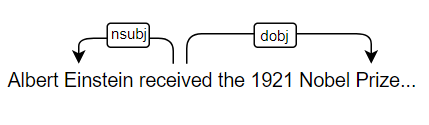
\includegraphics[width=.5\textwidth]{Dependency_4.png}
    \label{Statement1}
\end{figure}

\textit{In 1945, after having been nominated by Albert Einstein, Pauli received the Nobel Prize in Physics 
for his "decisive contribution through his discovery of a new law of Nature, the exclusion principle 
or Pauli principle".}

\begin{figure}[H]
    \centering
    \captionsetup{justification=centering}
    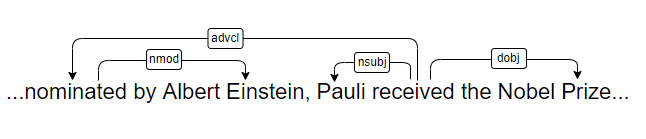
\includegraphics[width=.5\textwidth]{Dependency_2.png}
    \label{Statement2}
\end{figure}

\subsection{Topic terms based on word coherence}

Given a list of potential topic terms, \DeFacto\ identifies topic terms based on equations \ref{f:ttProp}, \ref{f:ttTitleProp} and \ref{f:ttComp}. These equations are only taking the document frequencies of terms within the set of documents retrieved for the given triple into account. The comparison in equation~\ref{f:ttComp} makes sure that a topic terms normalized document frequency is higher in the sub set of documents containing the triples \textit{subject} or \textit{object} in the title than in the set of all retrieved documents. A drawback of this approach is its focus on the set of documents retrieved for the given triple. A term could fulfil equation~\ref{f:ttComp} but could have an even higher document frequency outside of the retrieved document set. Apart from that, other terms that are helpful might be rejected.

In \FactCheck, we use the approach of word set coherences~\cite{roder2015exploring}. Given the list of potential topic terms, we calculate coherence values for these terms and the subject and object labels respectively. We select all terms whose coherence value is greater than a certain threshold and use them as topic terms.\footnote{For our experiments, we are using $0.2$ as threshold for the coherence value.}

For our experiments we use The normalized pointwise mutual information (NPMI) coherence~\cite{aletras2013evaluating} defined as the average NPMI value of all word pairs of the given word set. The NPMI value of a word pair $w_i$ and $w_j$ is defined as
\begin{equation}
NPMI(w_i, w_j)=\left(\frac{\log\left(\frac{P(w_i,w_j) + \epsilon}{P(w_i)P(w_j)}\right)}{\log \left(P(w_i,w_j) + \epsilon\right)} \right)
\end{equation}
where $\epsilon=10^{-12}$ and $P(w_i)$,$P(w_j)$ as well as $P(w_i,w_j)$ are probabilities gathered from the English Wikipedia using a sliding window of 10 words~\cite{roder2015exploring}. After all the topic terms are identified, we determine the trustworthiness features of documents as described in \DeFacto\ (see Section \ref{DeFacto-architecture}).

\section{Experimental setup and datasets}
\label{sec:expSetup}
In this section, we describe how we set-up the reference corpora and give details about the datasets we are using for our experiments.

\subsection{Reference corpora}

For our experiments, we used two reference corpora---ClueWeb and the English Wikipedia.

ClueWeb is created from raw web pages of the original ClueWeb12 corpus.\footnote{\url{https://lemurproject.org/clueweb12/}} Clue\-Web12 is a collection of web pages crawled from February to May 2012. They are stored using the WARC file format---an ISO standard file format that defines a structure for storing multiple resources collected from Web and other sources in a single file. As a first step, the WARC files are processed to remove all the HTML tags and metadata such as images and links. We then extract relevant information such as pageid, text, URL and the page title. Note that, we apply a threshold on length of the text and discard the web pages containing text shorter than 200 characters. In addition, we also use the pagerank information provided by the ClueWeb page rank\footnote{\url{http://www.lemurproject.org/clueweb12/PageRank.php}}. The extracted information along with pagerank is used to generate plain text documents. We generated approximately 420 million documents from the information extracted from the dataset of 5.4TB.

The second, smaller corpus is created by extracting plain text from English Wikipedia articles. It comprises 5.4 million plain text documents. 

All documents of ClueWeb and Wikipedia were indexed separately using Elasticsearch on a cluster of 7 nodes with a combined storage capacity of 15TB and computing capacity of 32GB RAM per node.

\subsection{Datasets}\label{subsec:Datasets}

For training and testing the classification model, positive and negative facts are required. Therefore we used two different datasets for our experiment---FactBench from \cite{gerber2015defacto} and the BPDP dataset created by us.

FactBench is a multilingual benchmark dataset for the evaluation of fact validation algorithms\cite{gerber2015defacto}.\footnote{\url{https://github.com/SmartDataAnalytics/FactBench}} All the facts in FactBench are automatically extracted from DBpedia and Freebase for 10 relations\footnote{\textit{award}, \textit{birthPlace}, \textit{deathPlace}, \textit{foundationPlace}, \textit{leader}, \textit{team}, \textit{author}, \textit{spouse}, \textit{starring}, \textit{subsidiary}} and stored in the form of RDF models. The facts are validated manually by three independent human annotators. FactBench is divided into train and test sets both containing positive and negative facts. The positive facts are generated by issuing SPARQL and MQL queries and selecting the top 150 results for each relation. The negative facts are derived by modifying positive facts. Given a KB $K$, let $S$ and $O$ be the set of all subjects and objects respectively in $K$. Let $P$ be set of all properties. Let triple $X=(s,p,o)$ represent a positive example in $K$ and $r$ a function which randomly selects an element from the given set. The following negative facts sets are generated corresponding to $X$ while still following domain and range restrictions.\\
\begin{tabular*}{\textwidth}{@{}lll@{}}
\textbf{Domain}: & $\{(s', p, o) $&$\mid s'=r(S), (s', p, o) \notin K \}$ \\
\textbf{Range}: & $\{(s, p, o') $&$\mid o'=r(O), (s, p, o') \notin K \}$ \\
\textbf{Domain-Range}: & $\{(s', p, o') $&$\mid s'=r(S), o'=r(O), (s', p, o') \notin K \}$ \\
\textbf{Property}: & $\{(s, p', o) $&$\mid p'=r(P), (s, p', o) \notin K \}$ \\
\textbf{Random}: & $\{(s', p', o') $&$\mid s'=r(S), p'=r(P), o'=r(O), (s', p', o') \notin K \}$ \\
\textbf{Mix}: & \multicolumn{2}{l}{This set is built by randomly selecting 20\% of the triples of each of}\\
              & \multicolumn{2}{l}{the above sets.} \\
\end{tabular*}\\

In each set of our experiment, FactCheck contains 1500 positive and 1500 negative examples. Note that, in each set we use same positive examples and the generated negative examples as described. All the facts in individual set are separated in to train and test sets each containing equal number of positive and negative examples. \\

The Birth Place/Death Place (BPDP) dataset is created by us. It is based on the observation that some fact checking approaches only check whether subject and object have a relation to each other. However, the type of the relation, i.e., whether it matches the property of the given fact, is not always taken into account. Therefore we create false facts with two entities that already have a similar relation to each other. To this end, we query DBpedia for persons which have their birth and death places in two different countries. We sort this list descending based on the probability of randomly choosing the person as described in \cite{Hare2017}. Two researchers check this list to make sure that the countries are different and not simply renamed because of historical events. The first 103 correct persons the two researchers agree on are chosen for the dataset. For each person, four facts are added to the dataset. Two facts have the correct birth and death place while the other two facts are generated by swapping birth and death place. Overall, the BPDP dataset comprises 412 facts separated in a train and a test set each containing an equal number of positive and negative facts.\footnote{The dataset is available at \url{https://hobbitdata.informatik.uni-leipzig.de/FactCheck/}.}

\subsection{Preparations}
%\todo{This section is not really "Training" and it is focusing too much on %FactBench. It has to be rewritten.}

For the experiments, \DeFacto\ and \FactCheck\ are trained on the train part of the dataset used in the experiment. This includes the generation of feature vectors for training classification models. These are used to train models for four different classifiers---J48, Simple Logistics, Naive Bayes and sequential minimal optimization (SMO)---of the Weka machine learning toolkit~\cite{weka2016}. A ten-fold cross validation is performed on the training examples. Once the final models are created, we generate the feature vectors for facts from the test set before classifying each single fact to be either true or false.

We carried out experiments for \DeFacto\ and \FactCheck\ using all subsets of FactBench as well as ClueWeb and Wikipedia as reference corpora. For the BPDP dataset, only experiments with Wikipedia as reference are carried out. Note that for a fair comparison, we extended \DeFacto\ to enable it to use our ClueWeb and Wikipedia indexes as reference corpora.

The classification results are evaluated using precision, recall, F1-measure, ROC-AUC as well as root mean square error (RMSE). Because of the limited space only a selected subset of the experiment results will be presented and discussed in the following section.\footnote{All results are available in our appendix which can be accessed at \url{https://hobbitdata.informatik.uni-leipzig.de/FactCheck/iswc2018-appendix.pdf}.}

\section{Results and discussion}
\label{sec:results}

The aim of our experiments is to answer the following three questions.
\begin{description}
 \item[Q1:] What is the impact of the corpus size on the classification accuracy?
 \item[Q2:] What is the quantitative improvement in performance of \FactCheck\ compared to \DeFacto\ due to the additional features?
 \item[Q3:] How does feature sub-sets influence the classification performance?
\end{description}

\begin{comment}
Table \ref{table:FactCheck_Mix} shows the classification performance of \FactCheck\ on \textbf{Mix} set and ClueWeb corpus. Given, \textbf{Mix} set is a heterogeneous collection of negative facts, F-Measures upto \textbf{0.885} for J48 indicate \FactCheck\ is effective at classifying positive and negative facts. Moreover, overall results of \FactCheck\ on other sets of training and testing examples shows that the framework is in general stable on all sets. In addition to overall quantitative evaluation, we also aim to answer the following questions.

\begin{table}
\caption{Classification results for \FactCheck\ on \textbf{Mix} set and ClueWeb corpus}
\label{table:FactCheck_Mix}
\centering
\begin{tabular}{lccccc}
    \toprule
    &\multicolumn{5}{c}{\FactCheck}\\
    &\textbf{P}&\textbf{R}&\textbf{F1}&\textbf{AUC}&\textbf{RMSE}\\
    \midrule
    J48 & 0.891 & 0.885 & \textbf{0.885} & 0.925 & 0.210\\
    Simple Logistics & 0.893 & 0.883 & 0.883 & \textbf{0.955} & 0.287\\
    Naive Bayes & 0.808 & 0.760 & 0.760 & 0.869 & 0.475\\
    SMO & 0.885 & 0.871 & 0.871 & 0.877 & 0.359\\
    \bottomrule
    
\end{tabular}
\end{table}
\end{comment}

\subsection{ \textbf{Q1:} Corpus size}

To answer \textbf{Q1}, we compare the results of both systems on the \textbf{Mix} sub set of FactBench using ClueWeb and Wikipedia as reference corpora. Tables~\ref{table:Defacto_Mix} and~\ref{table:FactCheck_Mix} show the results of \DeFacto\ and \FactCheck, respectively. The F-Measures of both systems are higher for all four classification algorithms when using the larger ClueWeb corpus. For the best classifiers, the F1-score increases by 0.027 for \DeFacto\ and 0.048 for \FactCheck, respectively. The reason for this improvement is that, for the majority of positive facts the number of source documents found in ClueWeb is higher compared to Wikipedia. Our inspection also shows that, for the DBpedia relations \textit{foundationPlace} and \textit{subsidiary}, the source documents for facts corresponding to these relations are not present in Wikipedia. However, sources for the same facts are found in ClueWeb owing to its large document collection.

\begin{table}
\footnotesize
\setlength{\tabcolsep}{1.5pt}
\caption{Classification performance of \DeFacto\ on the \textbf{Mix} sub set for the two reference corpora.}
\label{table:Defacto_Mix}
\begin{tabular*}{\textwidth}{lcccccccccccc}
    \toprule
    &\multicolumn{5}{c}{\textbf{Wikipedia }} & & \multicolumn{5}{c}{\textbf{ClueWeb}}\\
    &\textbf{P}&\textbf{R}&\textbf{F1}&\textbf{AUC}&\textbf{RMSE}&&\textbf{P}&\textbf{R}&\textbf{F1}&\textbf{AUC}&\textbf{RMSE}\\
    \midrule
    J48 & 0.809 & 0.802 & \textbf{0.803} & 0.827 & 0.392 && 0.832 & 0.830 & \textbf{0.830} & 0.829 & 0.384\\
    Simple Logistics & 0.795 & 0.784 & 0.784 & \textbf{0.847} & 0.394 && 0.819 & 0.818 & 0.818 & \textbf{0.871} & 0.378\\
    Naive Bayes & 0.726 & 0.600 & 0.554 & 0.820 & 0.620 && 0.762 & 0.740 & 0.740 & 0.863 & 0.480\\
    SMO & 0.787 & 0.777 & 0.777 & 0.782 & 0.471 && 0.821 & 0.820 & 0.820 & 0.816 & 0.424\\
    \bottomrule
\end{tabular*}
\end{table}

\begin{table}
\footnotesize
\setlength{\tabcolsep}{1.5pt}
\caption{Classification performance of \FactCheck\ on the \textbf{Mix} sub set for the two reference corpora.}
\label{table:FactCheck_Mix}
\begin{tabular*}{\textwidth}{lcccccccccccc}
    \toprule
    &\multicolumn{5}{c}{\textbf{Wikipedia }} & & \multicolumn{5}{c}{\textbf{ClueWeb}}\\
    &\textbf{P}&\textbf{R}&\textbf{F1}&\textbf{AUC}&\textbf{RMSE}&&\textbf{P}&\textbf{R}&\textbf{F1}&\textbf{AUC}&\textbf{RMSE}\\
    \midrule
    J48 & 0.840 & 0.837 & \textbf{0.837} & 0.825 & 0.391 && 0.891 & 0.885 & \textbf{0.885} & 0.925 & 0.299\\
    Simple Logistics & 0.836 & 0.835 & 0.835 & 0.883 & 0.368 && 0.893 & 0.883 & 0.883 & \textbf{0.955} & 0.288\\
    Naive Bayes & 0.768 & 0.684 & 0.659 & \textbf{0.894} & 0.555 && 0.808 & 0.760 & 0.760 & 0.869 & 0.475\\
    SMO & 0.826 & 0.825 & 0.825 & 0.825 & 0.4187 && 0.885 & 0.871 & 0.871 & 0.877 & 0.358\\
    \bottomrule
\end{tabular*}
\end{table}

\subsection{\textbf{Q2:} comparison of \FactCheck\ and \DeFacto}

Tables~\ref{table:Defacto_Mix} and~\ref{table:FactCheck_Mix} already showed that \FactCheck\ performs better than \DeFacto\ on the \textbf{Mix} sub set for both reference corpora. \FactCheck s F1-score is 0.034 and 0.055 points higher compared to \DeFacto\ when using Wikipedia and ClueWeb, respectively.

From \cite{gerber2015defacto} it is known that the \textbf{Property} sub set is the most difficult part of FactBench. Table~\ref{table:Propert_Set} shows the results for both system using the ClueWeb reference corpus. Again, it can be seen that \FactCheck\ clearly outperforms \DeFacto\ by 0.109 in terms of F1-measure and 0.084 in terms of AUC. A comparison with other FactBench sub sets shows that while \DeFacto\ is stable at classifying positive and negative examples on the other sets, its ability to classify facts corresponding to the \textbf{Property} is limited. This is due to the fact that the classification features in \DeFacto\ merely check for the presence of \textit{property} patterns in the proof phrases and fail to consider their relation with the \textit{subject} and \textit{object} label of the input triple. As shown in Section~\ref{subsec:Dependency_feature}, given the input triple and extracted proof phrases, none of features used in \DeFacto\ can effectively distinguish between the two example phrases. However, with the Dependency Parse feature of \FactCheck\ we particularly pay attention to the relations between \textit{subject}, \textit{property} and \textit{object} of the input triple while confirming facts from sentences. This enables \FactCheck\ to detect false facts even if the subject and object have a relation to each other.

\begin{table}
\footnotesize
\setlength{\tabcolsep}{1.5pt}
\caption{Classification performance of \FactCheck\ and \DeFacto\ on the \textbf{Property} sub set using the ClueWeb reference corpus.}
\label{table:Propert_Set}
\begin{tabular*}{\textwidth}{lcccccccccccc}
    \toprule
    &\multicolumn{5}{c}{\textbf{\FactCheck}} & & \multicolumn{5}{c}{\textbf{\DeFacto}}\\
    &\textbf{P}&\textbf{R}&\textbf{F1}&\textbf{AUC}&\textbf{RMSE}&&\textbf{P}&\textbf{R}&\textbf{F1}&\textbf{AUC}&\textbf{RMSE}\\
    \midrule
    J48 & 0.819 & 0.819 & \textbf{0.819} & \textbf{0.865} & 0.374 && 0.713 & 0.703 & 0.700 & 0.758 & 0.452\\
    Simple Logistics & 0.806 & 0.805 & 0.805 & 0.860 & 0.381 && 0.709 & 0.700 & 0.700 & \textbf{0.781} & 0.441\\
    Naive Bayes & 0.677 & 0.660 & 0.660 & 0.747 & 0.551 && 0.661 & 0.654 & 0.650 & 0.724 & 0.519\\
    SMO & 0.812 & 0.812 & 0.812 & 0.812 & 0.434 && 0.720 & 0.710 & \textbf{0.710} & 0.719 & 0.530\\
    \bottomrule
\end{tabular*}
\end{table}

This observation is supported by the comparison of the system results for the BPDP dataset. Although the dataset has been created to be even more challenging than the \textbf{Property} sub set of FactBench \FactCheck\ still reaches a high F1-measure which is 0.133 above the best F1-measure reached by \DeFacto \ as shown in  Table~\ref{table:FactCheck_BPDP}. This underpins \FactCheck s advantage over similar systems.

\begin{table}
\footnotesize
\setlength{\tabcolsep}{1.5pt}
\centering
\caption{Classification results of \FactCheck\ and \DeFacto\ on BPDP dataset}
\label{table:FactCheck_BPDP}
\begin{tabular}{lcccccccccccc}
    \toprule
    &\multicolumn{5}{c}{\textbf{\FactCheck}} & & \multicolumn{5}{c}{\textbf{\DeFacto}}\\
    &\textbf{P}&\textbf{R}&\textbf{F1}&\textbf{AUC}&\textbf{RMSE}&&\textbf{P}&\textbf{R}&\textbf{F1}&\textbf{AUC}&\textbf{RMSE}\\
    \midrule
    J48 & 0.814 & 0.811 & \textbf{0.811} & 0.878 & 0.368 && 0.691 & 0.678 & \textbf{0.678} & 0.715 & 0.494\\
    Simple Logistics & 0.792 & 0.783 & 0.782 & \textbf{0.922} & 0.348 && 0.626 & 0.623 & 0.623 & \textbf{0.729} & 0.487\\
    Naive Bayes & 0.800 & 0.760 & 0.760 & 0.869 & 0.475 && 0.623 & 0.623 & 0.622 & 0.68 & 0.579\\
    SMO & 0.811 & 0.811 & 0.811 & 0.811 & 0.434 && 0.682 & 0.673 & 0.673 & 0.673 & 0.497\\
    \bottomrule
\end{tabular}
\end{table}

\subsection{\textbf{Q3:} Feature sub-set analysis}

The third aim was to check which of the features used by \FactCheck\ is helpful for the classification of facts. Therefore we use sub-set evaluation techniques offered by Weka.\footnote{We used the evaluators \textit{WrapperSubsetEval}, \textit{ClassifierSubsetEval}, \textit{FilteredSubsetEval}, \textit{CfsSubsetEval} and \textit{ConsistencySubsetEval}.}
These evaluation techniques are used to search for the best feature combination for \textbf{Mix} sub set using the ClueWeb as reference corpus.
As classifiers we use J48 and the Simple Logistics owing to their performance on the selected set. 
%All experiments are performed using classifier that combine individual proof scores and trustworthiness scores. 
The results of the experiment show that J48 and Simple Logistics achieve F-measures of up to 0.898 and 0.892, respectively, when an optimized set of features is used. The sub-sets of features selected for the classifiers are shown in Table \ref{table:Subset_Eval1}.
It is worth noticing that both classifiers are using at least 2 of the topic-based measures relying on our newly introduced definition of topic words.
Only the features \textit{domain \& range verification} and \textit{statistical triple evidence} are missing in both lists.
However, this could be caused by the usage of the FactBench dataset. Since the creators of the dataset made sure that the domain and range of the properties are not violated, the domain \& range verification is not helpful for this dataset but might still be useful in other cases.
A similar effect can be assumed for the statistical triple evidence feature where subjects and objects of a false fact with valid classes with respect to domain and range of the facts property lead to $PMI$ values which can not be distinguished from the values of true facts.


\begin{table}
\footnotesize
\setlength{\tabcolsep}{2pt}
\caption{Feature sub-sets selected by J48 and Simple Logistics}
\label{table:Subset_Eval1}
\centering
\begin{tabular}{lp{1cm}l}
    \toprule
    {\textbf{J48}} & & {\textbf{Simple Logistics}}\\
    \midrule
    Total hit count & & Pagerank max\\
    Pagerank max & & Pagerank sum\\
    Topic Coverage & & Total hit count\\
    Topic Majority in Web & & Topic Coverage\\
    Total number of proofs & & Topic Majority in Web\\
    Total positive evidence score & & Topic Majority in Search\\
    Total negative evidence score & & Total number of confirming proofs\\
    & & Total positive evidence score\\
    & & Total negative evidence score\\
    \bottomrule
\end{tabular}
\end{table}

\section{Conclusion and Future work}
\label{sec:conclusion}

In this paper, we presented \FactCheck---a fact validation approach based on machine learning and textual evidence gathered from a reference corpus.
We showed that \FactCheck\ is able to outperform its predecessor \DeFacto\ on several datasets by up to 13.3\% F1-measure and 19.3\% AUC. Additionally, we analyzed the influence of the reference corpus size and the importance of the features used for the classification of facts.

\FactCheck\ does not rely on a costly Web search engine.
In the future, we want to use this advantage to create fact checking web services to enable access \FactCheck\'s functionality directly and to encourage other researchers to compare their own approaches with \FactCheck\ easily. Another interesting future work is to extend \FactCheck\ with more features and apply an ensemble learning instead of a single classifier.

\bibliographystyle{ACM-Reference-Format}
\bibliography{sample-bibliography}

\end{document}
